% CREATED BY DAVID FRISK, 2016
\chapter{Results}
\label{ch:results}

First the purpose of the paper is repeated to motivate the results obtained below. The main purpose of this paper is to investigate if  and how the VAHSS construction \ref{alg:VAHSS-HSS} can be extended with a range proof to ensure honest clients. Beside this main purpose the aim is also to provide an implementation of such a combined construction and to compare different range proofs and their compatibility to VAHSS. The results for there three questions will be given below.

\section{Combining}
The main result of this paper is that it is possible to combine a VAHSS construction as described in section \ref{sec:VAHSS} with a range proof to reduce the potential impact of malicious clients. Using range proofs (or set membership proofs) that assumes a Pedersen commitment the combining with the VAHSS construction becomes almost parallel in the scene that the VAHSS and range proof (or set membership proof) are run almost independent of each other. It was also found that the combination could be done without specifying the details about the range proof, hence any range proof that assumes a Pedersen commitment can be used, which leads to a highly flexible combination.  
%Note that although the construction does not specify which range proof that is used the implementation does due o the choice of group in the set up, the signature-based range proofs and set membership proof uses pairing friendly elliptic curve groups in the implementation which is not the case for Bulletproofs.

The main factor determining the suitability of different range proofs is their runtime and their possibility to be aggregated, since all can be combined using the same approach to the VAHSS construction. The two range proofs studied are Bulletproofs and signature-based range proofs and the runtime comparison between them presented in Table \ref{tab:runtime} showed that Bulletproofs were significantly faster both in the proof construction and verification algorithm. The insight that a straight forward combination as in Construction \ref{alg:VAHSS-HSS-RP} leads to that the verifier has to verify all range proofs separately lead to the attempt to aggregate the range proof, i.e combine the individual range proofs such that the verifier could instead verify one combined range proof. This can be compared to the the idea of the two algorithms \textbf{PartialProof} and \textbf{FinalProof} in the VAHSS construction, where the partial proofs are combined before the verification. It was found that the set membership proof and signature-based range proof could be partly aggregated such that the verifier only had to check one of the two equalities, in the algorithm \textbf{Verify} in construction \ref{alg:ZKSM} and \ref{alg:ZKRP}, for all clients and the other only once. The aggregation has been argued not ro weaken the completeness, soundness and zero knowledge requirements of the set membership and signature-based range proof.


\section{Runtime}
This is also confirmed to be the case when considering their difference in runtime when combined with a VAHSS, as seen in Table \ref{tab:BenchBP}. However above it has been discussed that set membership proofs and signature-based range proof can be partly aggregated, which would reduce the verification time.


  hence more suitable for using in server and client verifiable AHSS presented in Construction \ref{alg:VAHSS-HSS-RP}. 
  
  

\begin{table}
\caption{Timing in seconds for server and client verifiable-AHSS. Verification of clients is done using three different constructions namely  by implementing  Bulletproofs, signature based range proofs and set membership proofs}
\centering
\begin{tabular}{*{5}{c}}
\label{tab:BenchBP}
&  \textbf{Executer}   & \multicolumn{3}{c}{\textbf{Time}}   		\\ 
    										& 								& Bulletproofs  & Signature-based & Set membership \\	\hline
  GenerateShares 				&  client  					&   95 [$\mu$s]			 &96[$\mu$s]  &98 [$\mu$s]												\\ \hline 
  GenerateRangeProof  		&  clients  					&   53 [ms]				& 	241 [ms]	&66 [ms]			\\ \hline 
  PartialEval  						&  server  					&   78	[$\mu$s]				&72[$\mu$s]	 		&	71	 [$\mu$s]							\\ \hline 
  PartialProof 					&  server 					&   273[$\mu$s]						& 5249 [$\mu$s]			& 5255 [$\mu$s]				\\ \hline 
  FinalEval  						&  x  							&   689 [ns]						&655  [ns]				&			699  [ns]												\\ \hline 
  FinalProof  						&  x 							&   50	[$\mu$s]			&  114 [$\mu$s]	&				115 [$\mu$s]									\\ \hline 
  VerifyRP							&  x 							&   2979[ms]					&  &					9288 [ms]							\\ \hline 
  VerifyServers					&  x 							&   1672 [$\mu$s]					&		7990 [ms] 	&		7947 [$\mu$s]					\\ \hline 
\end{tabular}
\end{table}
 

To obtain the values in Table \ref{tab:BenchBP} the maximum upper bound for Bulletproof is $2^{n=8}=256$, which  is sufficiently large maximum upper bound  for the range $[18,200]$. However is would be interesting to investigate how the runtime of the verification in Construction \ref{alg:VAHSS-HSS-RP} is affected if this maximum bound of the range was increased. This is seen by the top curve in Figure \ref{fig:NrClients}. 
% The Bulletproofs has computational complexity $\mathcal{O}(log_2 n)$, thus an expected increase of a factor $5/3\:(=log_2\: 32/ log_2\: 8)$ would be expected, however in Figure \ref{fig:NrClients} an increase of a factor approximately $4$ is seen for the algorithm \texttt{Verify} in Construction \ref{alg:VAHSS-HSS-RP} when increasing $n$ form $8$ to $32$, why this result is obtained is not clear.
 An interesting remark is that  the runtime for Bulletproofs, when $n=32$, are longer then for set membership proofs independent of the number of clients considered and as mentioned earlier the runtime for verification using the set membership protocol in independent of both the size of the set and the values of the elements in the set. 
 \begin{figure}[]
\caption{TODO}
\label{fig:NrClients}
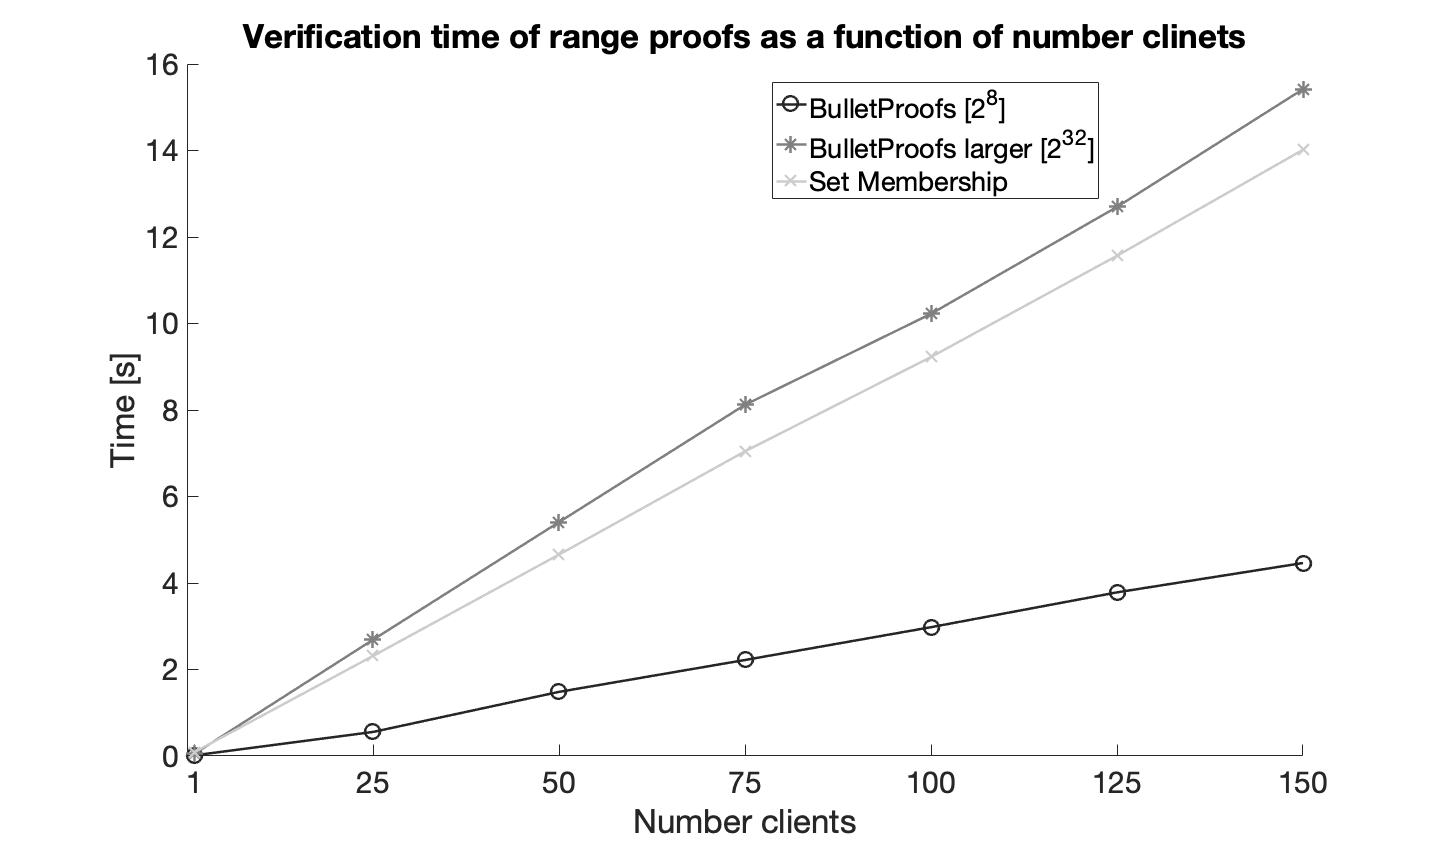
\includegraphics[width=\linewidth]{./figure/verification_nrClients.png}
\end{figure}

% 20 procnt speed up by aggrgegating. 
The aggregated version of the set membership and signature-based range proof has not been implemented thus result about how this aggregation affects the runtime can not be determined. In order to still get some idea of the runtime reduction, the algorithm \textbf{Verify} in Construction \ref{alg:ZKSM} was reduced to: 
\begin{itemize}
\item\text{\textbf{Verify} $(g,h,C,\textit{proof})\xrightarrow[]{}\{0,1\}$}
Check if $a \overset{?}{=} e(V,y)^c e(V,g)^{-z_x}e(g,g)^{z_\tau}$. If the equality holds the prover has convinced the verifier that $x\in\Phi$ return $1$ otherwise return $0$.
\end{itemize}
Then the runtime of this algorithm ran $100$ times, once for each clinet, was compared to the original version ran $100$ times. This gave the result that the modified version was approximately $20\%$ faster. This given some indication of the speed up obtained by aggregating since the equality check $D\overset{?}{=} C^ch^{z_\tau}g^{z_x}$ will only have to be ran once thus this runtime might be ignored in the context. 
